\documentclass[conference,usenames,dvipsnames]{IEEEtran}
\IEEEoverridecommandlockouts
% The preceding line is only needed to identify funding in the first footnote. If that is unneeded, please comment it out.
\usepackage{cite}
\usepackage{amsmath,amssymb,amsfonts}
\usepackage{algorithmic}
\usepackage{comment}
\usepackage{listings}
\lstset{language = C++}
\lstset{basicstyle=\ttfamily}
\usepackage{graphicx}
\usepackage[binary-units=true]{siunitx}
\sisetup{inter-unit-product =$\cdot$}
\usepackage{pgfplots}
\pgfplotsset{width=10cm,compat=1.9}
\usepgfplotslibrary{external}
\tikzexternalize
\usepackage{textcomp}
\usepackage{hyperref}
\hypersetup{
    colorlinks=true,
    linkcolor=blue,
    citecolor=Green,
    filecolor=magenta,      
    urlcolor=cyan,
}
\usepackage{xcolor}
\def\BibTeX{{\rm B\kern-.05em{\sc i\kern-.025em b}\kern-.08em
    T\kern-.1667em\lower.7ex\hbox{E}\kern-.125emX}}
\begin{document}

\newcommand{\citetemp}[1]{[\color{red}source\color{black}]}

\title{Comparing the Performance of RPT and DCPT Prefetching Algorithms}


\author{\IEEEauthorblockN{Aksel Torgerson
\IEEEauthorblockN{atorgerson@wisc.edu}
\IEEEauthorblockA{Faculty of Information Technology and E.E}
{Norwegian University of Science and Technology}\\
Trondheim, Norway}
\and
\IEEEauthorblockN{Marius C. K. Gulbrandsen}%Was something with this block
\IEEEauthorblockN{mariugul@stud.ntnu.no}
\IEEEauthorblockA{{Faculty of Information Technology and E.E.} \\
{Norwegian University of Science and Technology}\\
Trondheim, Norway}
}

\maketitle
% Get the reader to be interested in our paper. Short summary of our paper in an interesting way
\begin{abstract} \label{abstract}
In modern day computing, the \emph{memory gap} is one of the largest problems we face. As processor performance increases almost exponentially every year, memory access times do not. By implementing a prefetcher, we can decrease the impact of the memory gap and increase overall processor throughput. 

In this paper, we've explored how the implementation of a Reference Prediction Table (RPT) and Delta-Correlating Prediction Table (DCPT) compare when it comes to processor performance. The results showed that we were able to increase performance on average by 2\% for the RPT prefetcher and 10\% for the DCPT prefetcher. We were able to reduce misses by 18.7\% and 68.1\%, respectively.


\end{abstract}

\begin{IEEEkeywords}
cache, prefetcher, DCPT, RPT
\end{IEEEkeywords}

%%%%%%%%%%%%%%%%%%%%%%%%%%%%%%%%%%%%%%%%%%%%%%%%%%%%%
%% I have started to narrow down the abstract here %%
%%%%%%%%%%%%%%%%%%%%%%%%%%%%%%%%%%%%%%%%%%%%%%%%%%%%%

%In recent years, processor performance has increased almost exponentially, while memory access times have been increasing at a much slower rate. This has created what is known as \emph{the memory wall}. 

%A processor can handle an incredible amount of instructions per time unit, but, some of these instructions will require data from memory. The processor will need to stall until that data becomes available locally. To deal with this, and close the gap, prefetchers are used to collect the data before the processor requires it. 

%In this paper, we will explore how the implementation of a delta-correlating prediction table (DCPT) prefetcher affects processor performance. DCPT prefetchers are an improvement of RPT prefetchers and.. 

% A detailed introduction to the paper and concepts behind in
\section{Introduction} \label{sec:introduction}
In electrical and computer engineering, speed, power, and cost are the big three factors when it comes to designing processors. For decades, designers have been optimizing, analyzing, and testing the various trade-offs between the big three factors. Recently, processors have gained huge performance boosts, while memory access time has been mostly stagnant. This has led to the \emph{memory gap}\cite{Book}, as depicted in figure \ref{fig:memoryGap}. 

\begin{figure}[!htb]
    \centering
    \includegraphics[width = 8cm]{images/memoryGap.jpg}
    \caption{Processor-Memory Performance Gap\cite{Book}.}
    \label{fig:memoryGap}
\end{figure}

To deal with the increasing difficulties of the memory gap, techniques such as multi-level caching and prefetching are becoming more important in modern-day computing.
In processor design, the cache is perhaps the most important when it comes to making optimizations. Because the processor requires massive amounts of data throughout the life of a program, optimizing cache performance has an astronomical impact on the efficiency of said processor. Some of those cache optimizations are done directly in the cache by modifying cache parameters such as block size, associativity, and cache size, or, by dividing the cache up into multiple levels of storage such as L1, L2, and sometimes L3. However, interior cache architecture isn't the only way to optimize miss ratios and latency times.

Prefetching\cite{Prefetch} is a method of fetching cache blocks before they are needed, in an effort to close the memory gap. This allows future cache blocks to be simultaneously moved into the cache, while a prior instruction is being executed. In order for a prefetcher to be effective, it must accomplish two things. It needs to be able to predict which blocks are going to be needed in the future, while ensuring that those blocks are in the cache early enough to reduce the latency time, however, not too early so the cache becomes polluted. Those prefetched blocks could be evicted, effectively ruining the entire point of the prefetcher.

In this paper we are going to explore two data prefetching algorithms known as Reference Prediction Table\cite{RPT} and Data-Correlating Prediction Table\cite{grannaes}. Because hardware is used to implement these prefetchers, the cost and power consumption may be slightly higher, but it's a trade-off that will be worth it for the increase in speed. Theoretically, if we could have an algorithm to perfectly predict the needed blocks of data, we could completely eliminate latency in our design. However, this isn't possible because we cannot predict the future with 100\% certainty. Because we do not have actual hardware to implement on, a hardware-simulator was used to simulate the prefetchers.

Following in the paper, section \ref{sec:background} will discuss a variety of prefetchers and their performance. The methods used in securing good results is explained in section \ref{sec:methodology}. The coding of the DCPT algorithm and its implementation is described in section \ref{sec:implementation}, and the results can be found in section \ref{sec:results}. Discussion, related work, and conclusion follows in sections \ref{sec:discussion}, \ref{sec:related-work}, \ref{sec:conclusion}, respectively.

\newline
%\newline
\section{Background}\label{sec:background}
\subsection{Sequential Prefetching}
There are several implementations of prefetchers. The simplest form can be achieved with a sequential prefetcher\cite{prefetching}. These prefetchers tries to keep the cache pre-loaded with the data that is needed for the next instructions by fetching the next block upon a cache-miss. An improved version of the sequential prefetcher is the tagged sequential prefetcher. This adds an extra \emph{tag} to the cache blocks, and if there is a hit on a set tag, the prefetcher will fetch the next block.

\subsection{Reference Prediction Tables}
RPT prefetching involves the use of a large table to keep track of missed load instructions that have previously been called. 
\begin{figure}[!htb]
    \centering
    \includegraphics[width = 7cm]{images/RPTable.jpg}
    \caption{Organization of the Reference Prediction Table\cite{RPTimage}.}
    \label{fig:RPT Layout}
\end{figure}
Figure \ref{fig:RPT Layout} describes the layout of each table line. Each time a data block is missed, the address is stored in the ``Last Address'' field of the and the state is set to initial. The next time this data load results in a miss, the ``Last Address" is subtracted from the current address and the difference is stored in the ``Delta" field, and the state is now set to training. The third time this instruction results in a miss, the new delta is calculated, if the deltas are a match, the state is set to confirmed, and there is now a strided access pattern. The prefetcher can now load the next block into the cache prior to that load instruction being executed. 


\subsection{Program Counter/Delta-Correlation}
In the PC/DC method of prefetching, a Global History Buffer (GHB) is utilized to keep track of any cache hits or misses \cite{PCDC}. Figure \ref{fig:GHB Layout} describes how a GHB is structured.
\begin{figure}[!htb]
    \centering
    \includegraphics[width = 7cm]{images/GHBexample.png}
    \caption{Global History Buffer\cite{Book}.}
    \label{fig:GHB Layout}
\end{figure}
 Each time there is a miss, the index table will record the address of the respective block, and a pointer will be stored that points to the most recent miss from the same instruction. Each entry in the GHB also contains a pointer that references the next miss issued by the same instruction. Because we now have a ``chain" of pointers, we can traverse each one to see the pattern of the deltas between each address requested by each instruction that results in a miss. Now, the prefetcher will calculate said deltas, and store the values in the delta table. By traversing the stream of deltas, a pattern may be found. Once a pattern is detected, the prefetcher can start using the pattern to prefetch the predicted blocks.
 
%% State of the art subsection
\subsection{State of the Art} \label{subsec:state-of-the-art}
The DCPT functions similarly by finding a delta, or stride, between commonly accessed blocks. The DCPT method uses a table, similar to RPT. The table is indexed by the program counter (PC) of the instruction issuing a load. Table \ref{tab:DCPT} is an example of how a DCPT entry may look like.

\begin{table}[!htb]
\centering
\caption{Delta-Correlating Prediction Table.}
\label{tab:DCPT}
\begin{tabular}{ |c|c|c|c|c|c| } 
    \hline
    PC & Last Addr & Last Prefetch & Delta 1 & Delta n & Delta Pointer
    \\
    \hline
\end{tabular}
\end{table}

The last address field functions the same as RPT. The delta fields are initialized to 0, and the delta pointer field points to the head of the delta buffer. When a load instruction yields another miss, the delta is calculated like before, if the delta is 0, the buffer is not updated. After the buffer is updated, it is then traversed in reverse order to find a match to the most recently stored pair of deltas. Once a match is be found, the prefetcher adds the delta value to the last address, and stores this in the last prefetch field and sends it to a temporary prefetch candidate buffer. This process is repeated for each of the deltas following the matched pair. If the new prefetch candidate matches the last prefetch field, the entire content of the buffer is discarded up to this point.
Once the candidate buffer is finished, each entry is checked to see if it is in cache or not. If it is not, it is checked against the miss status registers to see if the block has been recently requested. Then, the candidate is checked against another buffer holding other prefetch requests that have yet to be completed. If the buffer is not full, the last prefetch field can be updated with the address, and the prefetch can take place.






\section{Methodology}\label{sec:methodology}
The prefetcher was simulated in a software environment to test the performance of the DCPT algorithm. Originally used to simulate computer networking, this simulator is very flexible and can be used to test a wide variety of applications.

    \subsection{Simulation Architecture}
    The DCPT prefetcher is run on a modified version of the M5 simulator, which is an open-source hardware simulator system \cite{M5}. It simulates an Alpha 21264 microprocessor, a super scalar, out-of-order, single core processor. The prefetcher runs on the L2 cache. Below are some of the important hardware specifications of this virtual system.
    
    \begin{table}[!htb]
    \centering
    \caption{M5 Hardware Specifications}
    \begin{tabular}{|l|l|}
    \hline
        L2 Cache Size    & \SI{1}{\mebi\byte}    \\
        Block Size       & \SI{64}{\byte}        \\
        Memory Bus Clock & \SI{400}{\mega\hertz} \\
        Memory Bus Width & \SI{64}{\bit}         \\
        Latency          & \SI{30}{\nano\second} \\
        \hline
    \end{tabular}
    \end{table}
    
    \subsection{Benchmarks}
    To evaluate the prefetcher we run it against the SPEC CPU2000 benchmark suite\cite{SPEC2000} which are CPU-intensive programs. Here are the relevant benchmarks used in the simulation. 
    
\begin{table}[!htb]
    \centering
    \caption{CPU2000 Simulation Benchmarks \cite{SPEC2000}}
    
    \begin{tabular}{ c|c|c} 
    \label{tab:my_label}
    Test & Type & Workload \\ 
    \hline
    ammp & float & Computational chemistry \\ 
    appulu & float & Partial differential equations \\ 
    apsi & float & Environmental modeling \\ 
    art & float & Neural network simulation \\ 
    bzip2 & int & Data compression \\ 
    galgel & float & Fluid dynamics \\ 
    swim & float & Water modeling \\ 
    twolf & int & Place and route simulation \\ 
    wupwise & float & Quantum chromodynamics \\ 
    \end{tabular}
\end{table}

Because each benchmark consists of a vastly different workload, you cannot expect one type of prefetcher to perform outstandingly on every test. Because we are not designing a prefetcher for a specific reason, we will be averaging all the scores from each benchmark and ranking the prefetcher based on an overall score.

\subsection{Evaluation}
    Following are the relevant equations that were used to evaluate the prefetcher implementation. 
    
    \begin{equation}
        Coverage = \frac{Eliminated\ misses}{Total\ misses\ without\ prefetching}
        \label{eq:coverage}
    \end{equation}
    
    Coverage, as shown in equation \ref{eq:coverage} is determined by taking the ratio of how many misses eliminated divided by the total number of misses without the implementation. It will roughly determine how well the prefetcher functions in regards to eliminated misses.
    
    \begin{equation}
        Accuracy = \frac{Eliminated\ misses}{Total\ number\ of\ prefetches}
        \label{eq:accuracy}
    \end{equation}
    
    Accuracy, as shown in equation \ref{eq:accuracy} is determined by taking the ratio of the eliminated misses over the total number of prefetches. The prefetchers could have a high coverage ratio, but it may be wasting resources by performing too many prefetches. In this case the accuracy is judged by measuring how many of the prefetches actually resulted in eliminated misses.
    
    %\begin{equation}
    %    Timeliness = \frac{On\ time\ %prefetches}{Useful\ prefetches}
    %   \label{eq:timeliness}
    %\end{equation}
    
    %Timeliness, as shown in equation \ref{eq:timeliness} is determined by taking the ratio of on time prefetches over those that were useful. For example, the prefetchers could be fetching all the correct blocks, however, they may be polluting the cache by fetching them too early. This can lead to a previously fetched block being replaced, and therefore nullifying any efforts of the prefetcher.

    For the statistics, the closer the ratio is to 1 is better. A perfect prefetcher would have a 1 for each ratio, but it is impossible to predict data with 100\% accuracy.
\section{Implementation}\label{sec:implementation}
The M5 simulator has three base functions that it calls: \lstinline{prefetch_init()}, \lstinline{prefetch_access()}, and \lstinline{prefetch_complete()}. In the following RPT and DCPT implementations, only the first two functions are utilized. 

\subsection{RPT}
During the initialization, a table is initialized that stores RPT entries. As shown above in figure \ref{fig:RPT Layout}, the table stores entries which consist of a program counter, previous address, a delta, and then pointers that point to the next and previous entries.

When the access function is called, it means that the L2 cache is called for a memory block. Once this happens, it is checked to see if it results in a miss. If so, the table is scanned to see if the block is already in the table. If it isn't in the table a new entry is generated that will replace the oldest entry if the table is full. Otherwise, it is added to the table and the respective pointers are updated. Once it is added it is updated with the program counter and the number of entries variable is incremented. 

After that, the new delta is calculated by subtracting the last address from the current address. If that new delta matches the one already in the entry, and the prospective block isn't already in the cache, and it's also not in the mshr queue, a prefetch is issued for that block. Then the delta and last address field are updated accordingly for that table entry.

\subsection{DCPT}
During initialization, a table is initialized that that stores DCPT entries. It also contains a variable to keep track of the amount of entries stored in the table. The entries consist of four fields as shown in figure \ref{tab:DCPT}, the program counter, the last address, the last prefetch address, and an array for the deltas. 

When the access function is called, the table is checked to see if that program counter has been referenced before. If the program counter is not in the table, and the table is full, the oldest entry is popped from the table to make room for the new entry. Otherwise, the new entry line is updated with the program counter and the memory address, and then it is pushed to the front of the table. Then, a pointer for the current entry is updated with the newest entry and the number of entries field in the table is incremented.
However, if the program counter was in the table it means that block has been accessed before and then delta calculation can begin. First, the new delta is calculated by subtracting the last address from the current address and then dividing it by the block size. Next, if the delta is not zero, it is added to the delta list. If the delta list was full, the oldest one is popped off and the new one is pushed on it. Then, the last address field is updated with the current address. Next, the last delta pair in the list is stored as variables, and the list is traversed from front to back to detect any matches in the delta buffer. If a match is found, the new address is calculated by adding all the deltas in between multiplied by the block size. Then, that address is pushed to a list of potential prefetch candidates. After that, the candidates need to be filtered to remove those already in-flight (not yet completed requests), in the mshr, and those already fetched in the cache. Then, loop through all the candidates, if it is not in-flight, in the mshr queue, or in the cache, push it to the prefetch list, and add it to the in-flight list. Then, set the last prefetch field in the current entry to point towards the candidate. Finally, loop through the prefetch list and issue a prefetch for each address in the list.

\section{Results}\label{sec:results}
 
\subsection{Overall Performance}
    Figure \ref{fig:OverallPerformance} shows the DCPT implementation preforming 10\% better than the included benchmark prefetchers. However, the RPT implementation achieves a speedup of only 2\%, slightly better than half of them.
    % Data
%----------------------------------------
\pgfplotstableread[row sep=\\,col sep=&]{
    prefetcher  & carT  \\
    This DCPT   & 1.10  \\
    This RPT    & 1.02  \\
    Tagged      & 1.01  \\
    SeqMiss     & 1.00  \\
    SeqAcc      & 1.01  \\
    RPT         & 1.06  \\
    DCPT-p      & 1.08  \\
    DCPT        & 1.05  \\
    AdapSeq    & 1.01  \\
    }\mydata

%Plot 
%----------------------------------------
\begin{figure}[!htb]
    \centering
    \begin{tikzpicture}
    \begin{axis}[
            ybar,
            ymin=.95,ymax=1.15,
            width = \textwidth/2,
            height = \textwidth/3,
            legend style={at={(0.5,1)},
                anchor=north,legend columns=-1},
            symbolic x coords={This DCPT, This RPT,Tagged,SeqMiss,SeqAcc,RPT,DCPT-p, DCPT, AdapSeq},
            xticklabel style={rotate=45},
            nodes near coords,
            nodes near coords align={vertical},
            xtick=data,
            %ylabel={Speedup},
        ]
        \addplot table[x=prefetcher,y=carT]{\mydata};
        
    \end{axis}
    \end{tikzpicture}
    
    \caption{Overall performance of different prefetchers}
    \label{fig:OverallPerformance}
\end{figure}

\subsection{Benchmarks}
    Figure \ref{fig:benchmarktest} shows how the RPT and DCPT prefetcher performs against each individual test. The DCPT prefetcher performs slightly worse on the \emph{twolf} test, but increases slightly until the \emph{wupwise} and \emph{ammp} tests, where it performs outstandingly well. RPT on the other hand has a negligible performance impact until run against the \emph{wupwise} and \emph{ammp} tests, where it performs slightly better.
    % Data
%----------------------------------------
\pgfplotstableread[row sep=\\,col sep=&]{
    bench   & DCPT & RPT  & nothing \\
    twolf   & 0.99 & 1.00 & 1.0 \\
    bzip2s  & 1.00 & 1.00 & 1.0 \\
    swim    & 1.01 & 0.99 & 1.0 \\
    bzip2g  & 1.03 & 1.01 & 1.0 \\
    bzip2p  & 1.04 & 1.01 & 1.0 \\
    art110  & 1.06 & 1.02 & 1.0 \\
    art470  & 1.06 & 1.02 & 1.0 \\
    apsi    & 1.09 & 1.01 & 1.0 \\
    applu   & 1.09 & 1.03 & 1.0 \\
    galgel  & 1.10 & 1.02 & 1.0 \\
    wupwise & 1.25 & 1.08 & 1.0 \\
    ammp    & 1.68 & 1.12 & 1.0 \\
    }\mydata

% Plot
%----------------------------------------
\begin{figure}[!htb]
\centering
\begin{tikzpicture}
    \begin{axis}[
            ybar,
            bar width=.1cm,
            width=\textwidth/2,
            height=\textwidth/3,
            %height=.5\textwidth/1,5,
            legend style={at={(0.5,1)},
                anchor=north,legend columns=-1},
            symbolic x coords={twolf, bzip2s, swim, bzip2g, bzip2p, art110, art470, apsi, applu, galgel, wupwise, ammp},
            xticklabel style={rotate=45},
            xtick=data,
            %nodes near coords,
            %nodes near coords align={vertical, rotate=90, anchor=west},
            ymin=.5,ymax=1.7,
            %ylabel={Speedup},
            %xlabel={Benchmark},
        ]
        \addplot table[x=bench,y=DCPT]   {\mydata};
        \addplot table[x=bench,y=RPT]    {\mydata};
        \addplot table[x=bench,y=nothing]{\mydata};
        \legend{DCPT, RPT, No Prefetch}
    \end{axis}
    \end{tikzpicture}
    \caption{Performance of DCPT vs RPT prefetchers}
    \label{fig:benchmarktest}
\end{figure}


\subsection{Statistics}
    Figure \ref{fig:statistics} shows the accuracy and coverage of the DCPT and the RPT prefetcher. These statistics can be calculated from equations (\ref{eq:coverage}) and (\ref{eq:accuracy}) which are explained in section \ref{sec:methodology}.
    % Data
%----------------------------------------
\pgfplotstableread[row sep=\\,col sep=&]{
    descr & DCPT & RPT            \\
    Accuracy     & 0.664  & 0.583 \\
    Coverage     & 0.471  & 0.10  \\
    }\mydata
%DCPT identified 2001231

% Plot
%----------------------------------------
\begin{figure}[!htb]
\centering
\begin{tikzpicture}
    \begin{axis}[
            ybar = 7pt,
            %bar width=.4cm,
            width=\textwidth/2,
            height=\textwidth/3,
            legend pos = north east,
            symbolic x coords={Accuracy, Coverage},
            xticklabel style={rotate=45},
            xtick=data,
            enlarge x limits = 0.7,
            nodes near coords,
            nodes near coords align={vertical},
            ymin=0, ymax=0.8,
            %ylabel={Speedup},
            %xlabel={Benchmark},
        ]
        \addplot table[x=descr,y=DCPT]{\mydata};
        \addplot table[x=descr,y=RPT]{\mydata};
        \legend{DCPT, RPT}
    \end{axis}
    \end{tikzpicture}
    \caption{Statistics for DCPT and RPT prefetchers}
    \label{fig:statistics}
\end{figure}


\subsection{Cache Size}
    Figure \ref{fig:cachesize} shows how the different implementations performed when the L2 cache size was changed. Because the speedup value is given in reference to a 1MB L2 cache, the relative speedups of using no prefetcher is also given. They were tested with a 1MB, 2MB, 4MB, 8MB, and 16MB L2 cache size. 
    \begin{figure}[!htb]
    \centering
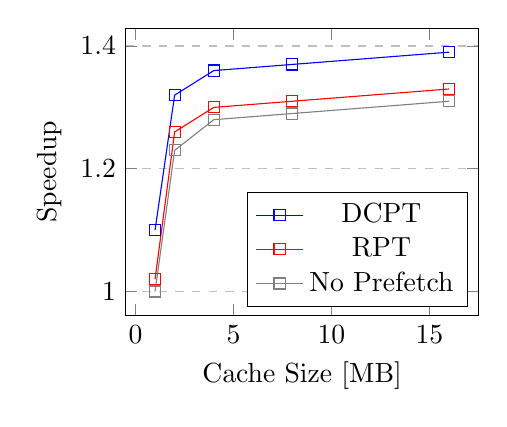
\begin{tikzpicture}
\begin{axis}[
    xlabel={Cache Size \SI{}{[\mega\byte]}},
    ylabel={Speedup},
    %xtick={0,1 ,2, 4, 8, 16},
    %ytick={0,0.5,1,1.5, 2},
    %nodes near coords,
    %nodes near coords align={vertical},
    legend pos=south east,
    ymajorgrids=true,
    grid style=dashed,
    width=\textwidth/2,
]
%DCPT
\addplot[
    color=blue,
    mark=square,
    ]
    coordinates {
    (1,1.1)(2,1.32)(4,1.36)(8,1.37)(16, 1.39)
    };
    
%RPT
\addplot[
    color=red,
    mark=square,
    ]
    coordinates {
    (1,1.02)(2,1.26)(4, 1.30)(8, 1.31)(16, 1.33)
    };
    
%No Prefetch
\addplot[
    color=gray,
    mark=square,
    ]
    coordinates {
    (1,1.0)(2,1.23)(4,1.28)(8,1.29)(16, 1.31)
    };

    \legend{DCPT, RPT, No Prefetch}
    
\end{axis}
\end{tikzpicture}
    \caption{Speedups compared to 1MB L2 cache with no prefetching}
    \label{fig:cachesize}
\end{figure}
    
\subsection{Delta Size}
    Figure \ref{fig:deltaEntries} shows how changing the amount of deltas per entry effects the relative speed up of the DCPT algorithm. Because RPT does not have a number of delta entries, it is not included in this graph.
    \begin{figure}[!htb]
    \centering
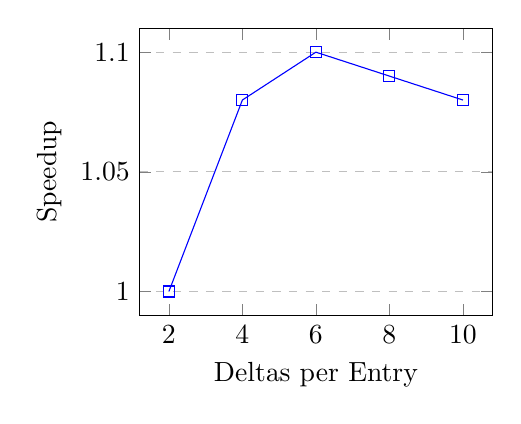
\begin{tikzpicture}
\begin{axis}[
    xlabel={Deltas per Entry},
    ylabel={Speedup},
    %xtick={0,1 ,2, 4, 8, 16},
    %ytick={0,0.5,1,1.5, 2},
    %nodes near coords,
    %nodes near coords align={vertical},
    legend pos=south east,
    ymajorgrids=true,
    grid style=dashed,
    width=\textwidth/2,
]
%DCPT
\addplot[
    color=blue,
    mark=square,
    ]
    coordinates {
    (2,1.00)(4,1.08)(6,1.1)(8,1.09)(10,1.08)
    };
    
    %\legend{DCPT, No Prefetch}
    
\end{axis}
\end{tikzpicture}
    \caption{Speedup of the DCPT algorithm with different amounts of deltas in each entry.}
    \label{fig:deltaEntries}
\end{figure}
\section{Discussion}\label{sec:discussion}
The first approach was to optimize the DCPT algorithm and analyze different implementations. This proved rather difficult, so the goal was changed to explore how a DCPT algorithm compares to an RPT algorithm. The DCPT implementation proved to have a marginally higher performance than the other algorithms as seen in figure \ref{fig:OverallPerformance}. However, on a few tests as seen in figure \ref{fig:benchmarktest}, the DCPT algorithm does not improve performance by a significant amount. In these cases RPT performance and DCPT performance varied by only by 1-2\% percent. Therefore when running these types of workloads, it is more efficient to run an RPT prefetcher because it uses less hardware and thus power.

As shown in figure \ref{fig:cachesize}, as the size of the cache increases, so does the average speedup compared to a cache with no prefetcher with a size of 1MB. This is expected of course, at least up until a certain point. In the tests ran, that limit was not observed, however, a strong stagnating trend was observed from 4MB cache size to 16MB cache size. In our prefetcher implementation, a 4MB cache size would yield the highest performance boost compared to the amount of hardware resources used.

After the implementation of the DCPT prefetcher was done, the max number of deltas in the table were modified as seen in figure \ref{fig:deltaEntries}. It was found that a delta array of length 6 yielded the highest performance boost. Because an array that is too short does not allow for as many delta correlations to be found, and an array length that is too long requires a longer period of time to iterate through and check for correlations, it seems that an array length of 6 is the optimal length.





%The implementation of the DCPT proves to have high performance compared to the benchmarks. However, the RPT implementation is not very efficient compared to the benchmarks, including the provided RPT prefetcher. This is likely due to a less efficient implementation of the algorithm, and also because RPT in general is a lower performing algorithm.

%This section might elaborate on alternative approaches that you have tried, but were not successful. It discusses weaknesses of your scheme and highlights the strong and weak points of your experimental setup.

\section{Related Work}\label{sec:related-work}

There has been other work put into improving algorithms for prefetching. M. Grannaes et.al\cite{grannaes} developed a DCPT algorithm that improves the performance by 43\%, using benchmarks running across SPEC2006.

D. Joseph et.al\cite{Markov} proposed a Markov prefetcher that would reduce data memory operations by 54\%. The predictions was based on identifying hidden markov models from observed sequences of cache misses.
%The related work section puts your paper into a research context. It mentions other research with similar goals or schemes and compares them to your work, highlighting the commonalities and differences. It also shows whether you have an overview of the research area.
\section{Conclusion}\label{sec:conclusion}
In this report, we have compared the RPT prefetching algorithm to the DCPT algorithm. The goal has been to see how well they both perform against each other by comparing the average speedup compared to using no prefetcher. 

Adjusting the number of deltas per entry proved that 6 deltas per entry is optimal. Too few deltas means that it does not allow for correlation to be found, and too many results in prefetches being too late.

Comparing RPT to DCPT has proved that the RPT algorithm had an overall geometric mean speedup by 2\% and the DCPT by 10\%. Despite the DCPT algorithm being more complex and consuming more resources, the speedup gained from it is worth the trade-off.

However, if a prefetcher was being designed for a specific purpose, such as place and route simulation, water modeling, or data compression, the DCPT algorithm would not be more efficient. Because the DCPT speedup gain was not significantly better than the RPT for those tests, it would be more efficient to use an RPT prefetcher in that case because the RPT prefetcher uses less hardware and consumes less power.

%\section*{Acknowledgment}\label{sec:acknowledgment}
Special thanks to Björn Gottschall for his help in all aspects of the paper as well as implementation.
\begin{thebibliography}{00}
%\bibitem{b2} T. Rosen, W.-S. Ong, and J. Upton, “ECE570 Final Paper,” Mar. 1996.
%\bibitem{b3} Asjad, Salahuddin \& Sildnes, Anders. (2016). Comparing Hardware Prefetching Schemes on an L2 Cache.


% The book
\bibitem{Book}Hennessy, J.L.; Patterson, D.A. Computer Organization and Design, 2nd ed. San Francisco: Morgan Kaufmann Publishers, 1997.

% chen and baer on RPT
\bibitem{Prefetch}T.-F. Chen and J.-L. Baer, “Effective hardware-based data prefetching
for high-performance processors,” Computers, IEEE Transactions on,
vol. 44, pp. 609–623, May 1995.

% RPT prefetching
\bibitem{RPT}D. Kim, “Extended data cache prefetching using a reference prediction table,” Ph.D. dissertation, 1997, aAI3114245.

% Grannes Jarhe and Natvig on DCPT
\bibitem{grannaes}Grannaes, Marius \& Jahre, Magnus \& Natvig, Lasse. (2011). Storage efficient hardware prefetching using delta correlating prediction tables. Journal of Instruction-Level Parallelism. 13. 1-16.

% Sequential prefetching


  
% Prefetching
\bibitem{prefetching} N. Honarmand, Class Lecture, Topic: "Memory Prefetching" Department of Computer Science, Stony Brook University, Stony Brook, New York, Spring, 2015.

% The image "RPT Layout"
\bibitem{RPTimage}
  S. VanderWiel and D. J. Lilja, "A Survey of Data Prefetching Techniques", 1999
% nesbit et al on DC/PC prefetching
\bibitem{PCDC}K. J. Nesbit and J. E. Smith, “Data cache prefetching using a global
history buffer,” High-Performance Computer Architecture, International
Symposium on, vol. 0, p. 96, 2004.

%NTNU M5 manual
\bibitem{M5}NTNU, M5 simulator system TDT4260 Computer Architecture User documentation, 
Trondheim, 2017.

% CPU 2000 benchmark suite
\bibitem{SPEC2000}SPEC CPU2000: Read Me First. [Online]. Available: https://www.spec.org/cpu2000/docs/readme1st.html. [Accessed: 18-Mar-2020].

% Markov
\bibitem{Markov}D. Joseph and D. Grunwald, “Prefetching using markov predictors,”
SIGARCH Comput. Archit. News, vol. 25, no. 2, pp. 252–263, May
1997.


%[#] A. Author, "Document title," Webpage name, Source/production information, Date of internet publication. [Format]. Available: internet address. [Accessed: Date of access].


\end{thebibliography}

\end{document}
